% =====================================================================
%  IT4868 - Web Mining - Project Proposal
%  Compiles with pdfLaTeX (Overleaf default)
% =====================================================================
\documentclass[11pt,a4paper]{article}

\usepackage[T1]{fontenc}
\usepackage[utf8]{inputenc}
\usepackage{mathptmx}
\usepackage[a4paper,margin=2.2cm]{geometry}
\usepackage{amsmath}
\usepackage{booktabs,tabularx,array}
\usepackage{enumitem}
\usepackage{xcolor}
\usepackage{tikz}
\usetikzlibrary{positioning,arrows.meta}
\usepackage{caption}
\usepackage{float}
\usepackage[hidelinks]{hyperref}
\usepackage{titlesec}

\setlist{itemsep=2pt,topsep=3pt}
\emergencystretch=3em
\sloppy
\titleformat{\section}{\large\bfseries}{\thesection.}{0.5em}{}
\titleformat{\subsection}{\normalsize\bfseries}{\thesubsection.}{0.5em}{}
\newcolumntype{Y}{>{\raggedright\arraybackslash}X}

\begin{document}

% ------------------------------ Title block ------------------------------
\begin{center}
  {\small SoICT -- HANOI UNIVERSITY OF SCIENCE AND TECHNOLOGY}\\[2pt]
  {\small IT4868 -- Web Mining \quad|\quad Lecturer: Dr. Duong Quang Huy}\\[10pt]
  {\large\bfseries PROJECT PROPOSAL}\\[8pt]
  {\LARGE\bfseries Semantic Matching and Ranking}\\[2pt]
  {\LARGE\bfseries for E-commerce Product Search}\\[6pt]
  {\normalsize Query--product ranking on the Amazon Shopping Queries (ESCI) dataset}\\[10pt]
  \begin{tabular}{ll}
    \toprule
    \textbf{Member} & \textbf{Student ID} \\
    \midrule
    Member 1 full name & ........ \\
    Member 2 full name & ........ \\
    Member 3 full name & ........ \\
    Member 4 full name & ........ \\
    \bottomrule
  \end{tabular}\\[6pt]
  {\small Hanoi, October 2026}
\end{center}

\begin{abstract}
\noindent In e-commerce search, a product can be an exact match for a query (Exact), a usable replacement (Substitute), an accessory (Complement) or irrelevant. We address Task~1 of the KDD Cup 2022 ESCI Challenge: given a query and its candidate products, rank them so that Exact products come first. We use the English part of the reduced dataset. Starting from lexical, dense and cross-encoder baselines, we plan to improve the cross-encoder with a richer product representation, a stronger backbone and a training objective suited to graded labels, and to add a second-stage re-ranker that uses information from the whole candidate list. Models are compared with nDCG against Amazon's published baselines.
\end{abstract}

% =====================================================================
\section{Introduction}
% =====================================================================
Product queries are short and full of specifications, brands and negations (``64gb'', ``without front cover''), and the words users type often differ from the words in product descriptions. Keyword matching therefore ranks highly products that share many words with the query but do not meet the need. Relevance is also not binary: a substitute is still useful when the exact product is missing, and an accessory is better than an unrelated item.

The Shopping Queries (ESCI) dataset~\cite{esci,aicrowd} provides such four-level labels for real Amazon queries, with official baselines and published competition solutions. It gives a well-defined problem, a public benchmark and reference results, and it connects the course topics of information retrieval (BM25, learning to rank, ranking metrics) with Transformer-based semantic matching.

% =====================================================================
\section{Problem Definition}
% =====================================================================
Each query $q$ comes with a candidate set $C_q$ returned by Amazon's search engine. Each pair $(q,p)$ has a human label $y \in \{E,S,C,I\}$ with the official gains $g(E)=1$, $g(S)=0.1$, $g(C)=0.01$, $g(I)=0$. Each product has a title, brand, color, bullet points and description.
\begin{itemize}
  \item \textbf{Input:} a query $q$ and its candidate products $C_q$.
  \item \textbf{Output:} a ranking of $C_q$.
  \item \textbf{Objective:} maximize nDCG with the ESCI gains.
\end{itemize}
\noindent\textbf{Example.} For \emph{``ipad case 8th generation without front cover''}, almost all candidates are iPad cases sharing the same words. A transparent back case is Exact, folio cases with a front cover are Substitutes, and a case for an older iPad model is Irrelevant. Telling them apart requires understanding the negation and the model numbers, not just word overlap.

\noindent\textbf{Scope.} Task~1 only, English (\texttt{us}) locale, reduced version. The candidates are given, so no retrieval over the full catalog is needed.

% =====================================================================
\section{Dataset}
% =====================================================================
We use the reduced version of the Shopping Queries Dataset~\cite{esci} (Apache-2.0), English part only. It consists of a table of labeled query--product pairs and a product table (482,105 products), joined on \texttt{product\_id}.

\begin{table}[H]
\centering
\caption{English portion of the reduced ESCI dataset (computed by the team).}
\label{tab:data}
\small
\begin{tabular}{@{}lrrcccc@{}}
\toprule
\textbf{Split} & \textbf{Queries} & \textbf{Pairs} & \textbf{E} & \textbf{S} & \textbf{C} & \textbf{I} \\
\midrule
Train & 20{,}888 & 419{,}653 & 43.3\% & 35.2\% & 4.5\% & 16.9\% \\
Test  & 8{,}956  & 181{,}701 & 43.9\% & 35.0\% & 4.5\% & 16.7\% \\
\bottomrule
\end{tabular}
\end{table}

\noindent Key observations:
(i) Exact and Substitute make up almost 80\% of the pairs, so the main difficulty is \textbf{separating E from S}, which often differ in a single attribute.
(ii) A query has about 20 candidates (median 16), so models that score every pair jointly with the query are affordable.
(iii) Product fields are often missing (no description for 48\% of products), and labels are noisy: near-identical products in the same list sometimes get different labels.
The reduced version is the official Task~1 data; the organizers removed ``easy'' queries from it, where most candidates are Exact and any ranking scores well.

\noindent\textbf{Splits.} Official train/test split; 10\% of the training queries are held out for validation, split by query.

% =====================================================================
\section{Related Work}
% =====================================================================
Amazon's baseline~\cite{esci} fine-tunes a small cross-encoder (MiniLM-L12) on the product title only and reaches 0.857 nDCG on English, against 0.675 for BM25. The top competition systems reached about 0.90 (all languages)~\cite{top1,second,zhichun,practice}. They share a few ingredients: large cross-encoders such as DeBERTa-v3~\cite{deberta} that read more product fields; pointwise objectives (regression on the gains, or 4-class classification turned into an expected gain), while pairwise training was reported not to help~\cite{second}; techniques against noisy labels~\cite{top1,zhichun}; and, in one solution, a gradient-boosting stage that combines model outputs with features of the whole candidate list~\cite{practice}. Large language models are not clearly better on this data~\cite{ebay}. We follow these directions under a student compute budget and study which of them matter.

% =====================================================================
\section{Proposed Approach}
% =====================================================================
\textbf{Baselines.} (B1) BM25 on the product text; (B2) a pre-trained bi-encoder, zero-shot; (B3) a reproduction of Amazon's cross-encoder baseline.

\noindent\textbf{Direction 1 -- A stronger cross-encoder.} Feed the brand, color and bullet points in addition to the title, since these hold the attributes that separate E from S, and replace MiniLM with \texttt{deberta-v3-base}.

\noindent\textbf{Direction 2 -- A training objective for graded labels.} Compare regression on the gains, classification with an expected-gain score, and a listwise loss (ListNet~\cite{listnet}) that trains on all candidates of a query together.

\noindent\textbf{Direction 3 -- Query-context re-ranking.} The cross-encoder scores each pair in isolation. A LightGBM~\cite{lightgbm} model re-ranks the list using the cross-encoder outputs together with list-level features (how a product's score compares with the other candidates, whether its brand is the most frequent one in the list) and simple match features (BM25, numbers and units, negated words). To avoid leakage, it is trained on out-of-fold cross-encoder predictions.

\begin{figure}[H]
\centering
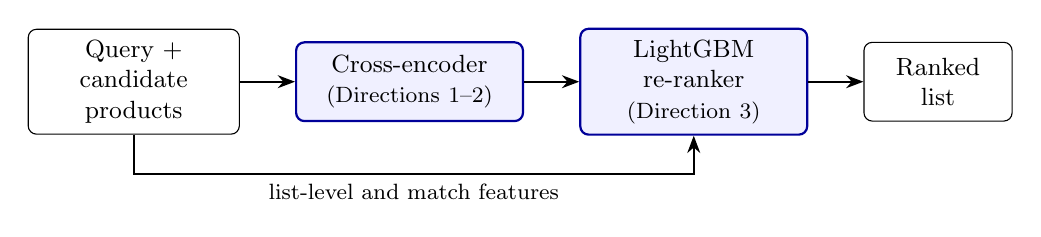
\begin{tikzpicture}[
  node distance=7mm,
  box/.style={draw, rounded corners=3pt, align=center, font=\small, minimum height=10mm, inner sep=4pt},
  acc/.style={box, draw=blue!60!black, fill=blue!6, thick},
  arr/.style={-{Stealth[length=2.2mm]}, semithick}]
  \node[box, text width=24mm] (in) {Query +\\candidate products};
  \node[acc, right=of in, text width=26mm] (ce) {Cross-encoder\\{\footnotesize (Directions 1--2)}};
  \node[acc, right=of ce, text width=26mm] (lgb) {LightGBM re-ranker\\{\footnotesize (Direction 3)}};
  \node[box, right=of lgb, text width=16mm] (out) {Ranked list};
  \draw[arr] (in) -- (ce);
  \draw[arr] (ce) -- (lgb);
  \draw[arr] (lgb) -- (out);
  \draw[arr] (in.south) -- ++(0,-5mm) -| node[pos=0.25, below, font=\footnotesize]{list-level and match features} (lgb.south);
\end{tikzpicture}
\caption{Planned pipeline.}
\end{figure}

\noindent\textbf{Priorities.} The \emph{core} plan is the three baselines and the three directions above. \emph{If time allows}, we will add handling of noisy labels (label smoothing, confident learning~\cite{cleanlab}), further objectives (ordinal~\cite{joint}, pairwise~\cite{pairwise}), a larger backbone and a small ensemble.

% =====================================================================
\section{Experiments and Evaluation}
% =====================================================================
\textbf{Planned experiments.}
\begin{enumerate}
  \item Compare the lexical, dense and cross-encoder baselines.
  \item Measure the effect of the richer product input and the stronger backbone.
  \item Compare the training objectives.
  \item Measure the gain of the query-context re-ranker over the cross-encoder alone.
  \item Error analysis by query type (negations, numbers and units, brands, query length) and on the worst queries.
\end{enumerate}

\noindent\textbf{Metrics.} nDCG over the full candidate list with the official ESCI gains (main metric), nDCG@10, MRR of the first Exact product, and the share of (Exact, Substitute) pairs ordered correctly. Differences are tested on per-query nDCG with a paired significance test. Our reproduced baselines are compared with the published BM25 (0.675) and cross-encoder (0.857) results; since Amazon's evaluation script swaps the gains of Substitute and Complement, we report both mappings for that comparison.

% =====================================================================
\section{Implementation and Plan}
% =====================================================================
\textbf{Tools.} Python, pandas, scikit-learn, \texttt{rank\_bm25}, PyTorch, HuggingFace Transformers, sentence-transformers, LightGBM; Google Colab / Kaggle GPUs; code on GitHub. We reuse Amazon's baseline code and pre-trained checkpoints; the evaluation module, input builder, training objectives, features and re-ranker are our own work.

\begin{table}[H]
\centering
\caption{Six-week plan (week 3 to the presentation in weeks 9--10).}
\small
\begin{tabularx}{\textwidth}{@{}c Y@{}}
\toprule
\textbf{Week} & \textbf{Work} \\
\midrule
1 & Data preparation, EDA, evaluation module, BM25 and bi-encoder baselines \\
2 & Reproduce Amazon's cross-encoder; richer product input \\
3 & DeBERTa-v3 backbone; comparison of training objectives \\
4 & Out-of-fold predictions, features, LightGBM re-ranker \\
5 & Error analysis; optional extensions; demo \\
6 & Report, slides, code clean-up \\
\bottomrule
\end{tabularx}
\end{table}

\begin{table}[H]
\centering
\caption{Planned task assignment.}
\small
\begin{tabularx}{\textwidth}{@{}l Y@{}}
\toprule
\textbf{Member} & \textbf{Responsibilities} \\
\midrule
Member 1 & Data, EDA, evaluation module, BM25 baseline \\
Member 2 & Bi-encoder baseline, features, LightGBM re-ranker \\
Member 3 & Cross-encoder baseline, input and backbone, GPU training \\
Member 4 & Training objectives, error analysis, demo \\
All & Report and slides \\
\bottomrule
\end{tabularx}
\end{table}

\noindent\textbf{Risks.} Limited GPU time: we explore with the small model and train the larger one only for selected settings. Gains over a strong baseline may be small: we rely on significance tests and per-query-type analysis rather than one overall number.

% =====================================================================
\begin{thebibliography}{99}\small\setlength{\itemsep}{0pt}\setlength{\parskip}{0pt}
\bibitem{esci} C.~K. Reddy, L.~M\`arquez, F.~Valero, N.~Rao, H.~Zaragoza, S.~Bandyopadhyay, A.~Biswas, A.~Xing, K.~Subbian. \emph{Shopping Queries Dataset: A Large-Scale ESCI Benchmark for Improving Product Search}. arXiv:2206.06588, 2022.
\bibitem{aicrowd} AIcrowd. \emph{ESCI Challenge for Improving Product Search}. \url{https://www.aicrowd.com/challenges/esci-challenge-for-improving-product-search}
\bibitem{top1} Q.~Zhang, Z.~Yang, Y.~Huang, Z.~Chen, Z.~Cai, K.~Wang, J.~Zheng, J.~He, J.~Gao. \emph{A Semantic Alignment System for Multilingual Query-Product Retrieval}. arXiv:2208.02958, 2022.
\bibitem{second} X.~Qin, N.~Liang, H.~Zhang, W.~Zou, W.~Zhang. \emph{Second Place Solution of Amazon KDD Cup 2022: ESCI Challenge for Improving Product Search}. KDD Cup 2022 Workshop.
\bibitem{zhichun} X.~Cui, W.~Xiong, S.~Wang. \emph{ZhichunRoad at Amazon KDD Cup 2022: MultiTask Pre-Training for E-Commerce Product Search}. KDD Cup 2022 Workshop.
\bibitem{practice} F.~Wu, Y.~Liu, R.~Gazo, B.~Bedrich, X.~Qu. \emph{Some Practice for Improving the Search Results of E-commerce}. KDD Cup 2022 Workshop.
\bibitem{ebay} C.~Palen-Michel, R.~Wang, Y.~Zhang, D.~Yu, C.~Xu, Z.~Wu. \emph{Investigating LLM Applications in E-Commerce}. arXiv:2408.12779, 2024.
\bibitem{deberta} P.~He, J.~Gao, W.~Chen. \emph{DeBERTaV3: Improving DeBERTa using ELECTRA-Style Pre-Training with Gradient-Disentangled Embedding Sharing}. arXiv:2111.09543, 2021.
\bibitem{listnet} Z.~Cao, T.~Qin, T.-Y.~Liu, M.-F.~Tsai, H.~Li. \emph{Learning to Rank: From Pairwise Approach to Listwise Approach}. ICML 2007.
\bibitem{lightgbm} G.~Ke, Q.~Meng, T.~Finley, T.~Wang, W.~Chen, W.~Ma, Q.~Ye, T.-Y.~Liu. \emph{LightGBM: A Highly Efficient Gradient Boosting Decision Tree}. NeurIPS 2017.
\bibitem{cleanlab} C.~G. Northcutt, L.~Jiang, I.~L. Chuang. \emph{Confident Learning: Estimating Uncertainty in Dataset Labels}. JAIR 70, 2021.
\bibitem{joint} L.~Chen et al. \emph{Joint Optimization of Relevance and Engagement in Multi-Task Ranking for E-Commerce with Efficient LLM Supervision}. SIGIR 2026. arXiv:2605.27704.
\bibitem{pairwise} F.~Durmus, H.~Saribas, S.~Aldemir, J.~Yang, H.~Cevikalp. \emph{Pairwise Ranking Loss for Multi-task Learning in Recommender Systems}. arXiv:2406.02163, 2024.
\end{thebibliography}

\end{document}
